%% ==============================
\chapter{Introduction}
\label{sec:introduction}
%% ==============================
Questions to ask:
\begin{enumerate}
    \item What is your research topic? (From wide to narrow scope)
    \item What is the research problem or gap in the field that this work aims to address?
    \item Why is this problem or gap important?
    \item What are the research questions or hypotheses? 
    \item What is the scope of your work? (What are the limitations?)
    \item How is the following work structured?
\end{enumerate}

\begin{enumerate}
    \item General field of path planning for mobile robots
    \item Problem of path planning in multi-floor environments
    \item Shared human-robot spaces
    \item Research question: How to plan in a multi-floor environment? And how to drive in public spaces with service robots?
    \item Significance: Many use cases in public spaces in large, complex hierarchical environments like hospitals.
    \item Development of a global planner plugin for straight and predictable paths in multi-floor environments.
    \item Structure of the thesis
\end{enumerate}

%% ==============================
\section{Motivation}
\label{sec:motivation}
%% ==============================
The research area of autonomous mobile robotics deals with all sub-areas that are necessary to ensure the required degree of autonomy and mobility for specific tasks. In addition to navigation and manipulation, this also includes the perception of the environment as well as the internal state. Autonomous mobile robots form a combination of the disciplines of electrical engineering, mechanical engineering and computer science. Computer science in particular is rapidly driving current developments. Complex algorithms for localisation and navigation enable the necessary mobility. Artificial intelligence offers robust methods for image processing, object recognition and voice control through neural networks and machine learning. According to the market research company Gartner, autonomous robotics is the most important strategic technological trend of 2019 \cite{cearley_gartner_2018} and number eight in 2020 \cite{david_cearley_gartner_2019} In recent years it has only been superseded by new developments in the field of AI. The market for professional service robots is growing rapidly. According to the International Federation of Robotics, the number of professional service robots sold in 2021 grew by 37 \% to a total of 121,000 units \cite{international_federation_of_robotics_world_2022}. The largest are of application is transportation and logistics. These are robots that mostly operate in strictly defined spaces separated from humans, for example robots for material logistics in warehouses or production facilities.

Especially in the application area of service robotics in shared human-robot spaces, tasks are becoming increasingly complex. The best-known are household robots for consumers that, for example, take care of vacuuming or mow the lawn. However, more extensive tasks such as support in everyday life by folding the laundry \cite{srivastava_tractability_2015} or assisting in the kitchen \cite{becker_pr2_2011}, can now also be taken over by assistance robots. The professional application of service robots is mostly limited to isolated tasks without the need to interact with humans. There are a few start-ups which are trying to establish service robots in public spaces as well \cite{kittmann_let_2015}. However, the development of service robots for public spaces is still in its infancy. The main reason for this is the complexity of the tasks and the environment. In addition to the technical challenges, there are also legal and ethical issues that need to be addressed.

%% ==============================
\section{Problem Statement}
\label{sec:problem_statement}
%% ==============================
Mobile robots are increasingly being used in large environments, such as hospitals, to improve efficiency and reduce human workload. However, navigating over multiple stories poses a significant challenge for mobile robots, as it requires a planner that can account for complex spatial configurations and still find the shortest path. Moreover, the planned path must be straight, deterministic and predictable for humans who could be walking in the same space as the robot. Therefore, the specific research problem addressed in this thesis is the development of a planner that can enable a mobile robot to navigate over multiple stories in complex environments, while ensuring a straight, deterministic and human-predictable path. 

The ability to navigate over multiple stories is important for mobile robots in large, complex environments, as it can significantly increase their utility and effectiveness. For instance, in hospitals, mobile robots could be used for tasks such as delivering medicines, transporting equipment, or guiding patients and visitors. Although for specific use-cases proprietary solutions exist, the lack of an open-source planner for multi-floor navigation is a major bottleneck in the development of mobile robots for service applications. Moreover, the need for a straight, deterministic and human-predictable path is essential for ensuring safety and reducing the risk of collisions or accidents in shared human-robot spaces.

The two main research questions addressed in this thesis are:
\begin{enumerate}
    \item How to navigate in complex multi-floor environments?
    \item How to plan paths that are straight, deterministic and human-predictable?
\end{enumerate}

The scope of this work is limited to the development of a planner that plans a priori with previously collected information, as opposed to a controller that follows the planned path and adapts to dynamic obstacles. The main assumption is that a map of the entire environment has been previously recorded and provides a complete representation of the plannable space.

%% ==============================
\section{Use case PeTRA}
\label{sec:use_case}
%% ==============================
The use case of this work is a mobile robot that is used to support staff with patient logistics in care facilities. This includes tasks such as delivering medicines and transporting a patient to examinations. This work is part of the \gls{petra} research project, which is funded by the \gls{bmbf} \cite{bmbf-internetredaktion_bekanntmachung_2018} and developed at the \gls{iras} of the \gls{hka}.

The daily routine in a hospital includes transporting patients from ward to examination. This manual transport is mostly performed by trained nurses, who are can not perform nursing activities while they are absent from the ward. To reduce transfer time, patients are moved through the hospital in beds, even though some of them would be able to walk by themselves. This transfer method neither promotes the patients' mobility nor allows them to decide for themselves whether and how they want to walk. "\Gls{petra} is designed to relieve caregivers of time-consuming and labor-intensive patient transport and give them more time for qualitative care" \cite{petra-konsortium_personen-transfer_2022}. To achieve this goal, an autonomous mobile robot was developed in collaboration with industry partners and three hospitals. \Gls{petra} offers different transfer modes, to adapt to each patients need, see figure  \ref{fig:multi_mobility_methods}. Autonomous patient transport is realized with sensory coupling for free walking or with the support of a rollator (center) and a modular platform for wheelchairs (left). This platform is used for safe wheelchair transport and can be coupled. In addition, an integrated robotic arm performs service tasks (right). These include, for example, the transport of drugs or blood samples between the storage area and the wards..

\begin{figure}[h]
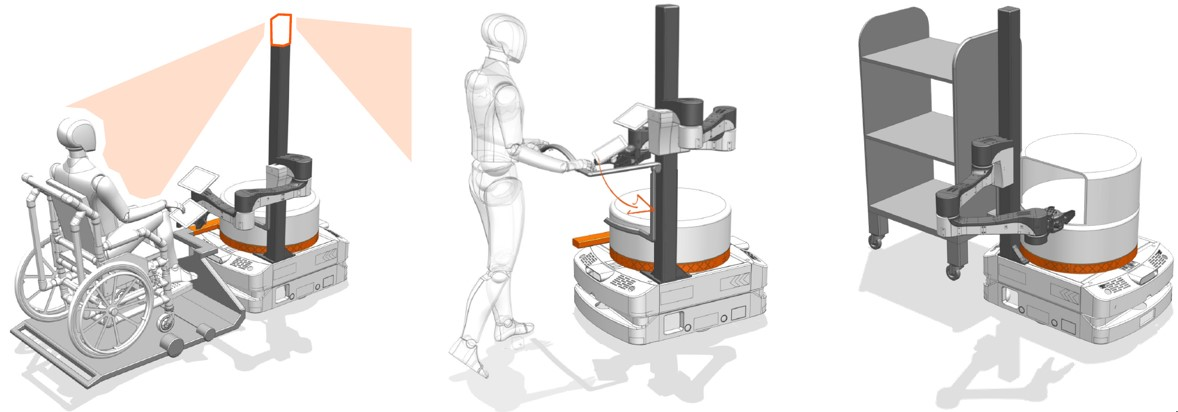
\includegraphics[width=\textwidth]{figures/20_state_of_the_art/PeTRA_transport_modes.jpg}
\caption[]{Multi-mobility methods of PeTRA: Wheelchair transport (left), sensory coupling (center) and material transport (right).}
\centering
\label{fig:multi_mobility_methods}
\end{figure}
To demonstrate the feasibility and economic viability of autonomous transports in hospitals \gls{petra} needs to be able to carry out jobs between arbitrary locations in this complex environment. This work enables \gls{petra} to navigate over multiple floors while following a predictable path.

%% ==============================
\section{Structure of this Thesis}
\label{sec:structure}
%% ==============================
The following work is structured as follows: Chapter \ref{sec:state_of_the_art} provides an overview of the state of the art in the field of multi-floor path planning for mobile robots. It also discusses the limitations of existing approaches. Chapter \ref{sec:methods} describes the methodology used to address the research questions. The concept of the graph-based planner is presented in Chapter \ref{sec:concept} followed by the implementation in Chapter \ref{sec:implementation}. This shows the approaches of creating a graph from a previously recorded map. Chapter \ref{sec:results} presents the results of the work. Chapter \ref{sec:discussion} discusses the results and provides recommendations for future work. Chapter \ref{sec:conclusion} concludes the thesis.